\documentclass[11pt]{article}

\usepackage[a4paper,margin=2.5cm]{geometry}
\usepackage{graphicx}
\usepackage{float}
\usepackage{booktabs}

\title{HPC: Labwork \#3}
\author{Nguyen Trong Minh}
\date{Tuesday, September 30, 2026 \\ SonTG}

\begin{document}

\maketitle

\section{Implementation}

The coding is quite simple. I replicate the grayscale conversion code using CUDA from the slides and also implement the same operation on the CPU. For each pixel, I take the average of the three RGB channels and use it as the value for all three output channels:

\[
    \mathrm{gray} = \frac{R + G + B}{3}.
\]

The input image has a shape of $1032 \times 1242 \times 3$. Before sending it to the GPU, I reshape it into a two-dimensional array where each row contains the three channels of one pixel. Each CUDA thread processes one pixel. A boundary check is used because the number of launched threads can be slightly larger than the number of pixels.

I then use \texttt{time.perf\_counter()} to measure the execution time across four block sizes for each CUDA run. I use 32, 64, 128, and 256 threads per block. The CPU version is run three times, and I use its mean execution time. I call \texttt{cuda.synchronize()} before stopping the GPU timer so that the measured value includes the actual kernel execution and not only the kernel launch.

\section{Output Images}

Both implementations produce the same grayscale result. The output arrays are reshaped back to the original image dimensions before they are saved as PNG files.

\begin{figure}[H]
    \centering
    \begin{minipage}[t]{0.48\textwidth}
        \centering
        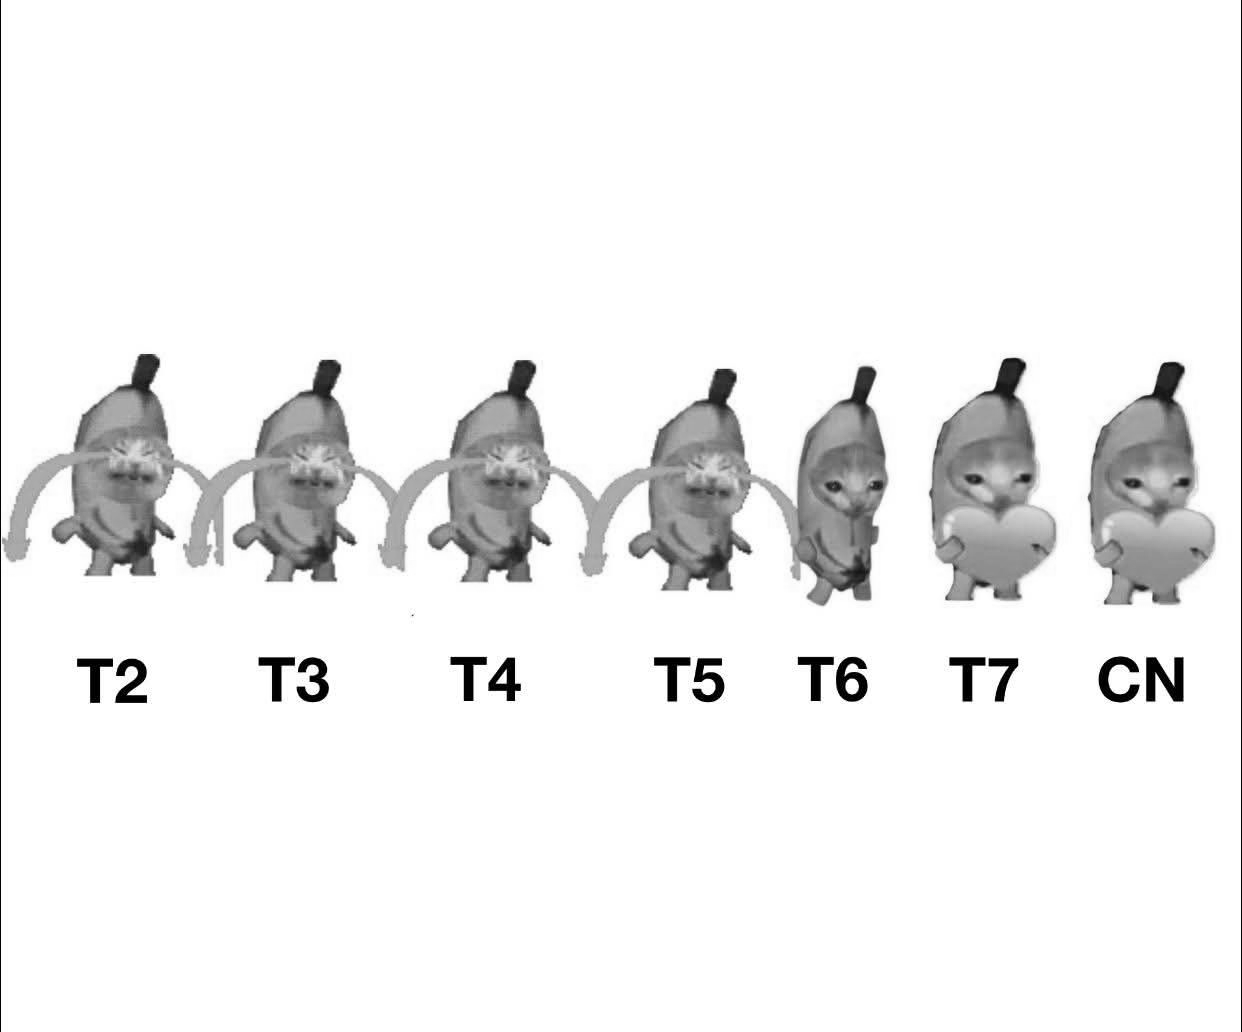
\includegraphics[width=\linewidth]{cpu_grey.png}
        \small CPU output
    \end{minipage}
    \hfill
    \begin{minipage}[t]{0.48\textwidth}
        \centering
        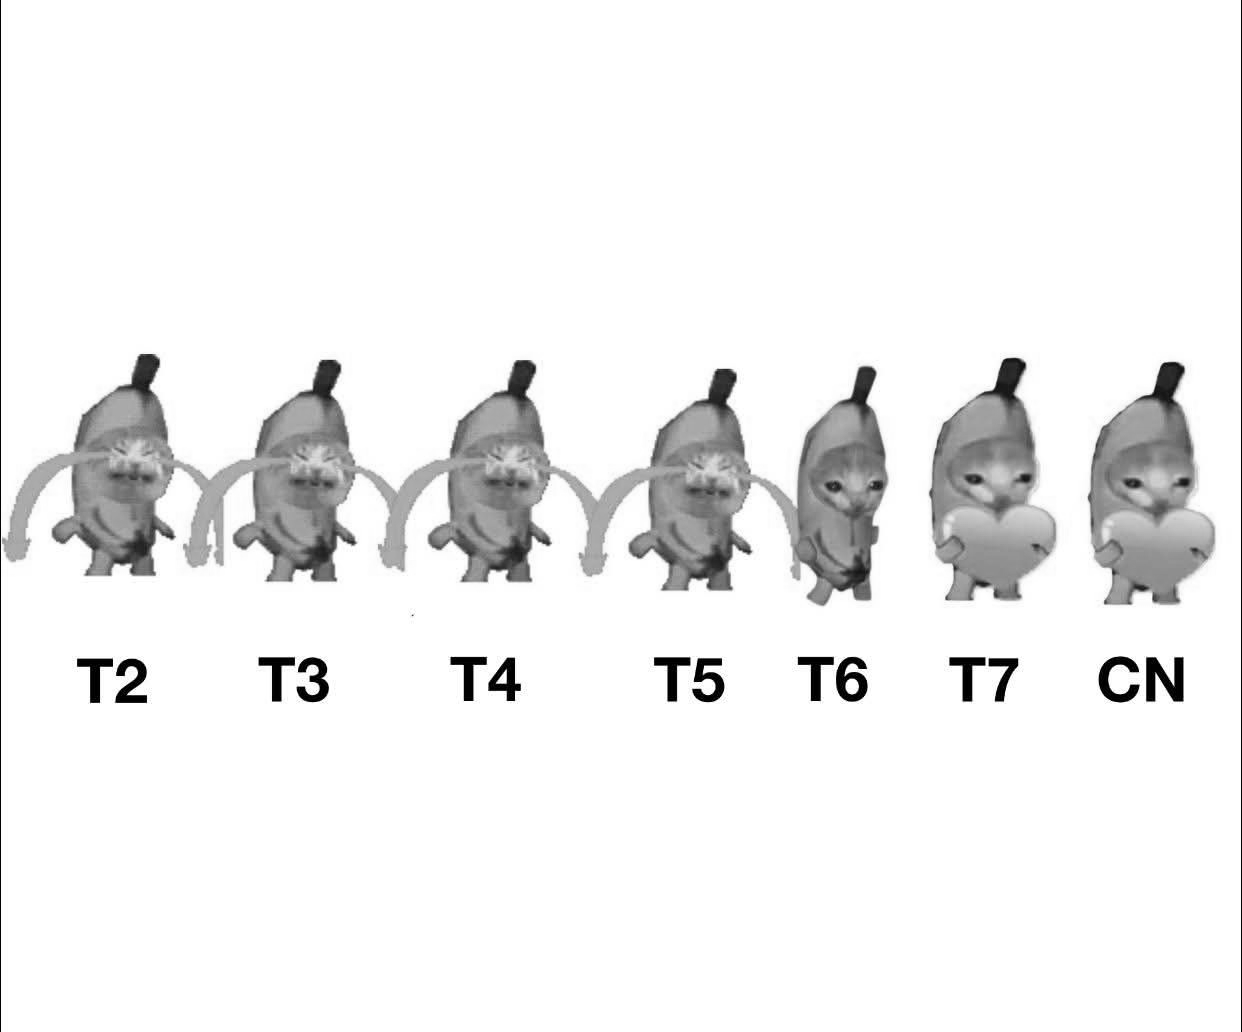
\includegraphics[width=\linewidth]{gpu_grey.png}
        \small GPU output
    \end{minipage}
    \caption{Grayscale images generated by the CPU and CUDA implementations.}
    \label{fig:outputs}
\end{figure}

\section{Result}

The timing result is shown in Figure~\ref{fig:timing}. A logarithmic scale is used because the GPU execution times are much smaller than the CPU execution time.

\begin{table}[H]
    \centering
    \begin{tabular}{lr}
        \toprule
        Configuration & Execution time (seconds) \\
        \midrule
        GPU, 32 threads per block  & $5.51 \times 10^{-4}$ \\
        GPU, 64 threads per block  & $4.32 \times 10^{-4}$ \\
        GPU, 128 threads per block & $4.21 \times 10^{-4}$ \\
        GPU, 256 threads per block & $4.27 \times 10^{-4}$ \\
        CPU                        & $1.22$ \\
        \bottomrule
    \end{tabular}
    \caption{Measured grayscale processing time.}
    \label{tab:timing}
\end{table}

\begin{figure}[H]
    \centering
    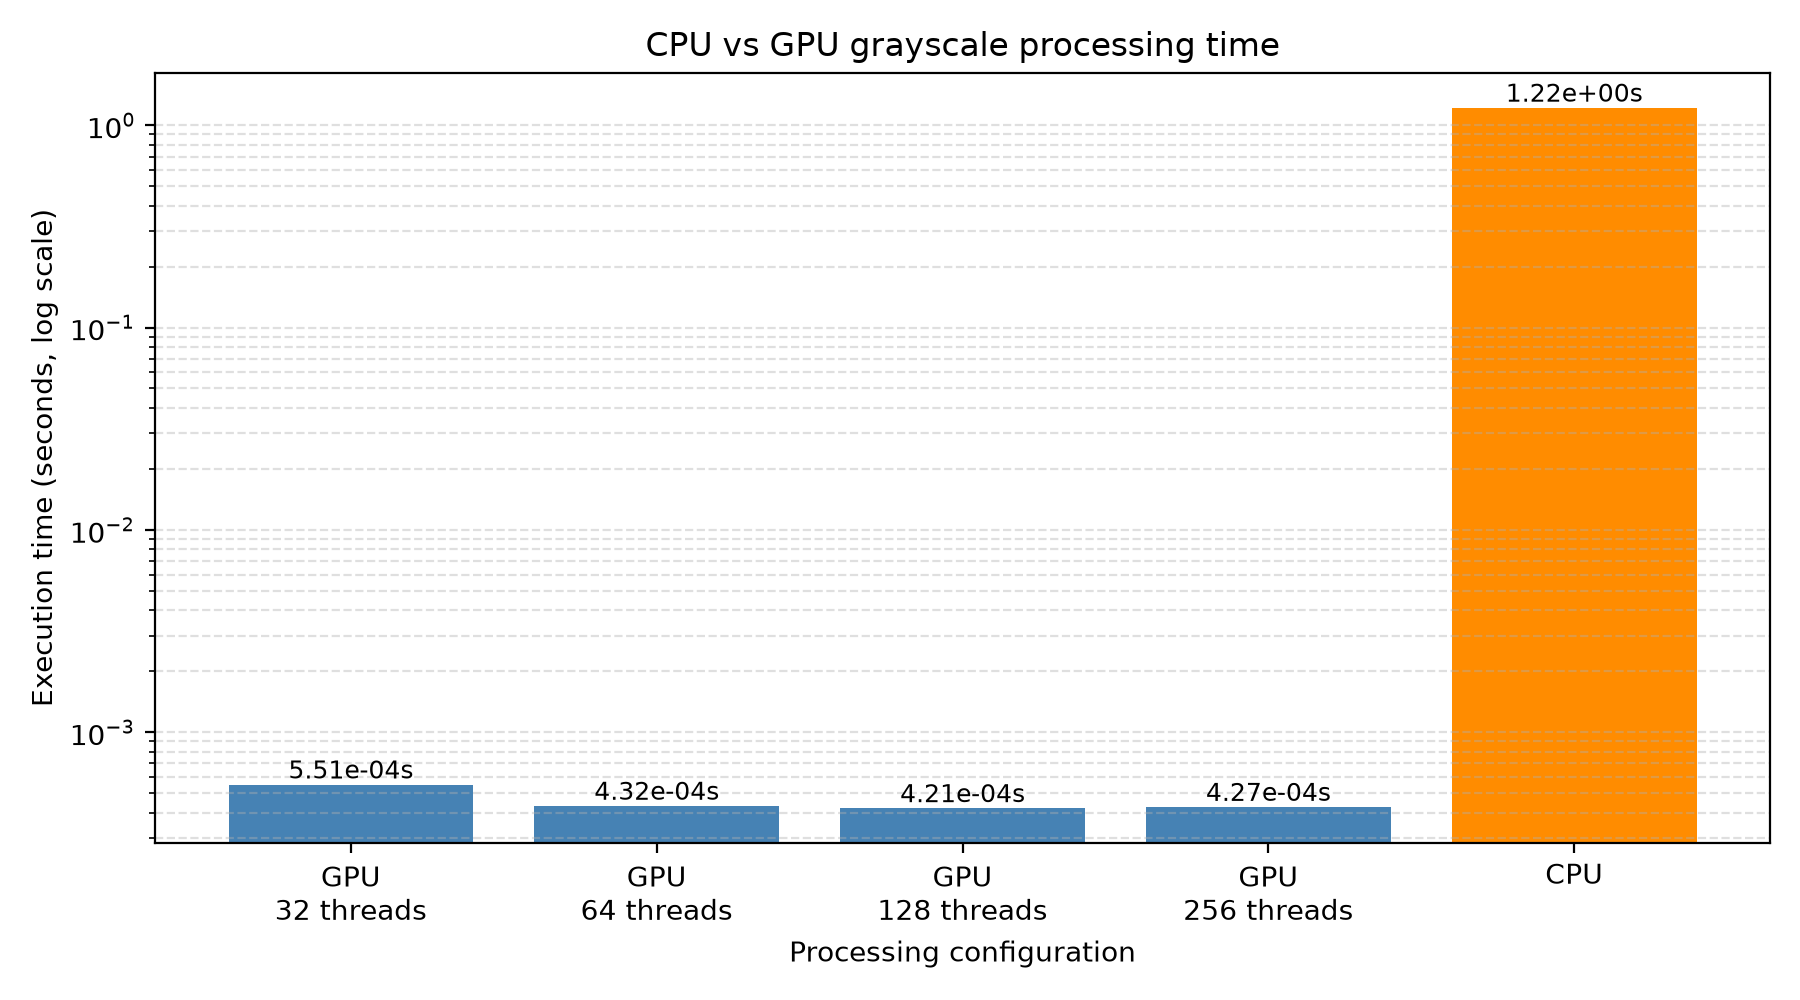
\includegraphics[width=0.82\textwidth]{execution_time.png}
    \caption{CPU and GPU execution time on a logarithmic scale.}
    \label{fig:timing}
\end{figure}

Using CUDA clearly gives a faster execution time compared with the CPU version. The fastest measured configuration is 128 threads per block at approximately $4.21 \times 10^{-4}$ seconds. The 64-thread and 256-thread configurations give very similar results, while 32 threads per block is slightly slower. This means that using fewer threads per block does not automatically make the program faster. The final performance depends on the scheduling and resource usage of the GPU.

For this image, the 128-thread configuration is approximately 2,900 times faster than the measured CPU implementation. However, the CPU code uses a Python loop, so this comparison includes Python interpreter overhead. The result demonstrates the benefit of processing many independent pixels in parallel, but it should not be treated as a comparison against an optimized vectorized CPU implementation.

\section{Conclusion}

The CPU and GPU implementations generate the same grayscale image, but the CUDA kernel completes the pixel processing much faster. Among the tested block sizes, 128 threads per block gives the lowest execution time. This labwork also shows that CUDA timing needs synchronization and that array shapes and bounds must be handled carefully when each thread processes one pixel.

\end{document}
